% =============================================
% CAPÍTULO 7 - MODELAGEM DO BANCO DE DADOS
% =============================================
\chapter{MODELAGEM DO BANCO DE DADOS}

Segundo Elmasri e Navathe (2011, p. 131), "Geralmente o termo aplicação de banco de dados refere-se a um banco de dados em particular e aos programas associados que implementam as consultas e atualizações dele". Com isso em mente, a modelagem do banco de dados se trata de uma fase indispensável do desenvolvimento de um produto. Ao se pensar em como será a estrutura de um banco e seus relacionamentos, é possível trazer à tona regras de negócios e comportamentos implícitos que poderiam não ser identificados ao não se passar por esse estágio antes do desenvolvimento do produto.

A plataforma adota uma estratégia de persistência poliglota, utilizando dois bancos de dados com propósitos distintos e complementares: o \textbf{PostgreSQL} para dados relacionais — como usuários, contas vinculadas, metas financeiras, consentimentos e registros de auditoria — e o \textbf{MongoDB} para dados semi-estruturados de alto volume, como transações e histórico financeiro. Essa separação permite otimizar cada banco para seu caso de uso específico, garantindo desempenho, escalabilidade e conformidade com a Lei Geral de Proteção de Dados (LGPD).

\section{Diagrama entidade relacionamento}

Na Figura \ref{fig:der_postgres} é apresentado o Diagrama de Entidade Relacionamento do banco de dados relacional (PostgreSQL), com seus principais atributos e seus respectivos relacionamentos, com identificação de entidades fortes e fracas.

\begin{figure}[H]
    \centering
    \caption{DER do sistema — PostgreSQL}
    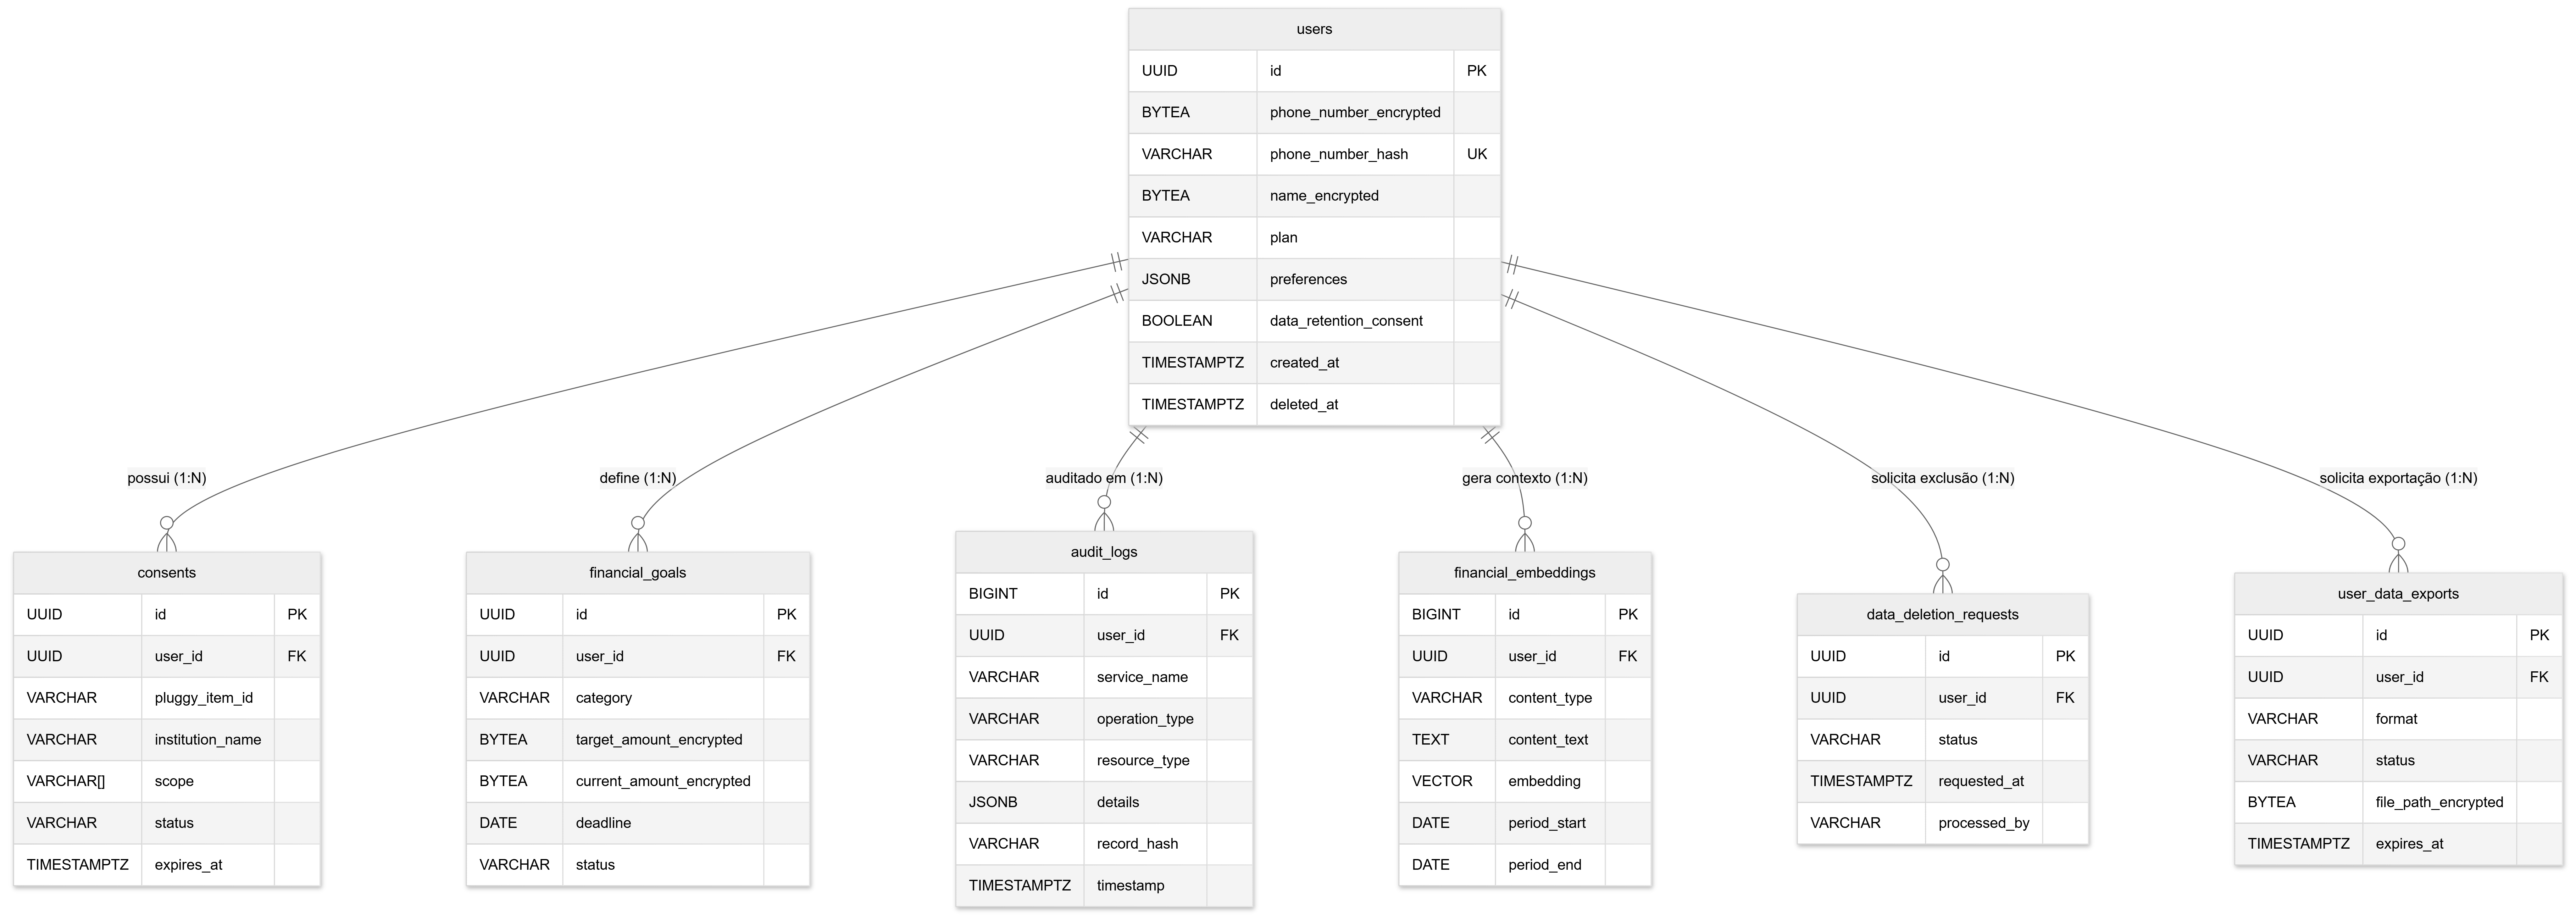
\includegraphics[width=\textwidth]{images/der_postgres.png}
    \label{fig:der_postgres}
    \fonte{Elaborado pelos autores (2026).}
\end{figure}

\section{Modelo entidade relacionamento}

O Modelo Entidade-Relacionamento (MER) é empregado para representar os elementos do mundo real por meio de entidades, as quais possuem atributos que descrevem suas características, e relacionamentos que estabelecem conexões entre essas entidades (OLIVEIRA, 2022).

Na Figura \ref{fig:mer_postgres} é apresentado o modelo de entidade relacionamento do banco de dados relacional com suas relações e atributos.

\begin{figure}[H]
    \centering
    \caption{MER do sistema — PostgreSQL}
    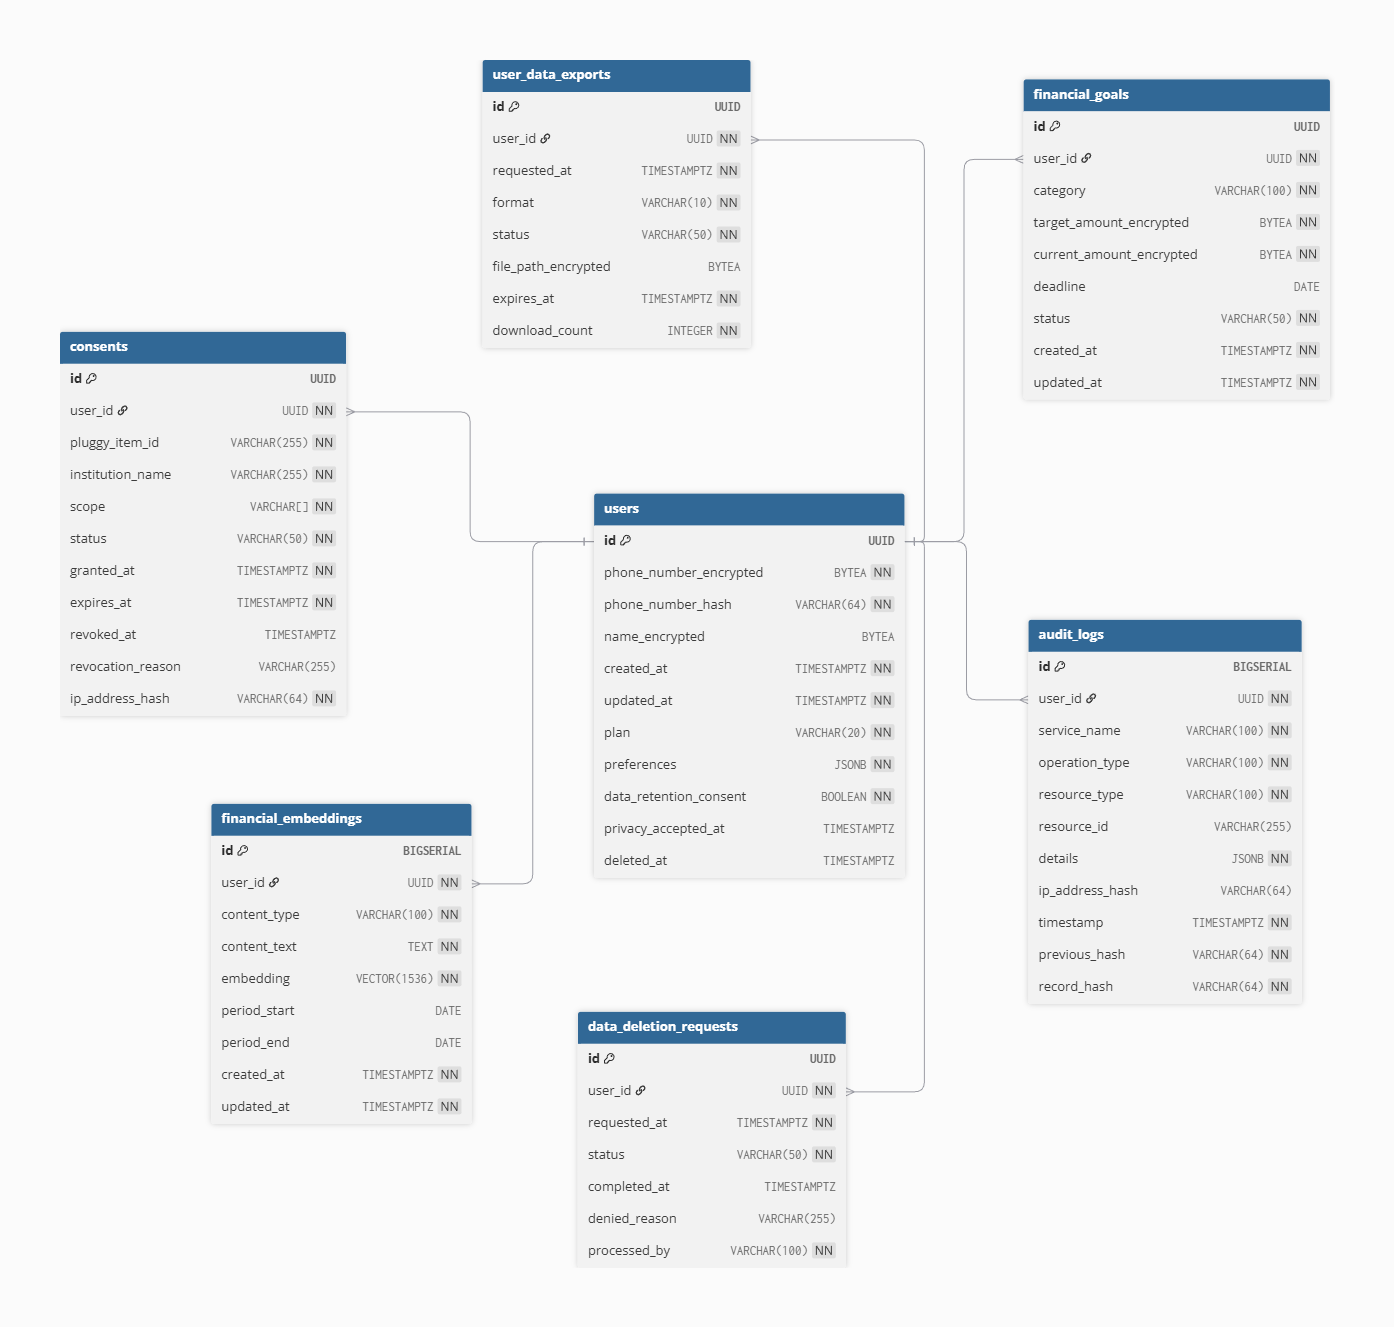
\includegraphics[width=\textwidth]{images/mer_postgres.png}
    \label{fig:mer_postgres}
    \fonte{Elaborado pelos autores (2026).}
\end{figure}

\section{Modelo de dados orientado a documentos}

O MongoDB é empregado para armazenar dados semi-estruturados de alto volume, como transações financeiras sincronizadas via Open Finance e o histórico financeiro dos usuários. A flexibilidade do modelo de documentos permite representar estruturas variáveis conforme o tipo de transação, sem a necessidade de migrações de esquema. Para garantir a conformidade com a LGPD, campos monetários e dados sensíveis são criptografados em nível de campo por meio da \textit{Client-Side Field Level Encryption} antes de serem persistidos.

Na Figura \ref{fig:mongo} é apresentado o modelo de dados orientado a documentos utilizado no MongoDB.

\begin{figure}[H]
    \centering
    \caption{Modelo de dados — MongoDB}
    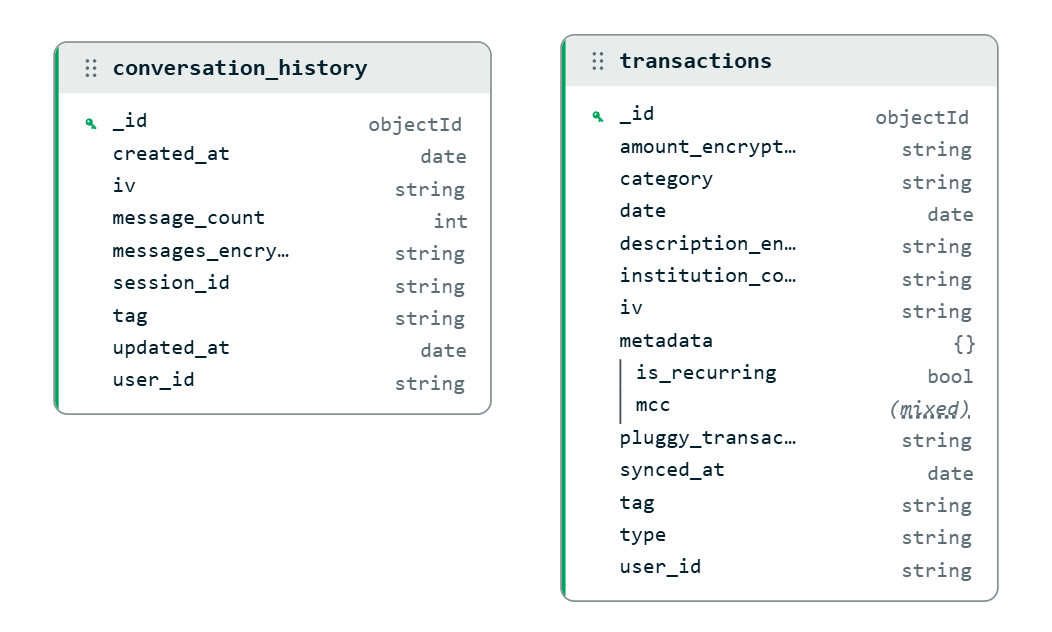
\includegraphics[width=\textwidth]{images/mongo.png}
    \label{fig:mongo}
    \fonte{Elaborado pelos autores (2026).}
\end{figure}
